\documentclass[a4paper, 10pt]{article}
\usepackage{../../CEDT-Homework-style}

\usepackage{amsmath}
\allowdisplaybreaks

\setlength{\headheight}{14.49998pt}

\begin{document}
\subject[2110203 - Computer Engineering Mathematics II]
\hwtitle{Signal 2}{}{Week 2}{6733172621 Patthadon Phengpinij}{ChatGPT (for\,\LaTeX\,styling and grammar checking)}


% ================================================================================ %
\section{Convolution}
% ================================================================================ %



% ================================================================================ %
%                                    Problem 01                                    %
% ================================================================================ %
\begin{problem}
Evaluate the convolution of the following signals
\end{problem}

% === Problem 1.1. === %
\begin{subproblems}[start=1]
    \item \( \textrm{rect} \paren{ \frac{t-a}{a} } * \delta (t-b) \)
\end{subproblems}

\begin{solution}
From the sifting property of the delta function, we have:
\[ f(t) * \delta(t - b) = f(t - b) \]

Applying this property to our problem, we get:
\[ \textrm{rect} \paren{ \frac{t - a}{a} } * \delta(t - b) = \textrm{rect} \paren{ \frac{(t - b) - a}{a} } = \textrm{rect} \paren{ \frac{t - (a + b)}{a} } \]

Thus, the result of the convolution is:
\[ \boxed{ \textrm{rect} \paren{ \frac{t - (a + b)}{a} } } \]

Using Python to verify this result, we can implement the convolution and plot the results.
The plot of the signal is shown below:
\begin{center}
    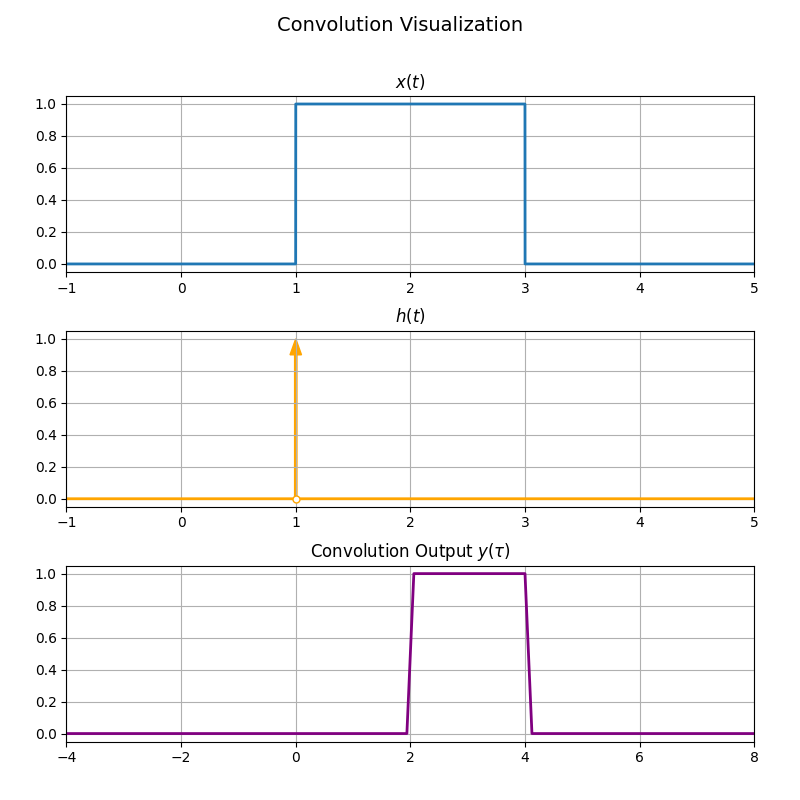
\includegraphics[width=0.7\textwidth]{images/problem_1_1_snapshot.png}
\end{center}
\end{solution}
% ==================== %

\newpage

% === Problem 1.2. === %
\begin{subproblems}[resume]
    \item \( \textrm{rect} \paren{ \frac{t}{a} } * \textrm{rect} \paren{ \frac{t}{a} } \)
\end{subproblems}

\begin{solution}
To evaluate the convolution of two rectangular functions, we start with the definition of the rectangular function:
\[ \textrm{rect} \paren{ \frac{t}{a} } = \begin{cases} 1 & \text{if } |t| \leq \frac{a}{2} \\ 0 & \text{otherwise} \end{cases} \]

The convolution of two functions \( f(t) \) and \( g(t) \) is defined as:
\[ (f * g)(t) = \int_{-\infty}^{\infty} f(\tau) g(t - \tau) \, d\tau \]

Applying this to our rectangular functions, we have:
\[
\begin{aligned}
    ( \textrm{rect} \paren{ \frac{t}{a} } * \textrm{rect} \paren{ \frac{t}{a} } )(t) &= \int_{-\infty}^{\infty} \textrm{rect} \paren{ \frac{\tau}{a} } \textrm{rect} \paren{ \frac{t - \tau}{a} } \, d\tau \\
    &= \int_{-\frac{a}{2}}^{\frac{a}{2}} \textrm{rect} \paren{ \frac{t - \tau}{a} } \, d\tau \\
    &= \int_{\max(-\frac{a}{2}, t - \frac{a}{2})}^{\min(\frac{a}{2}, t + \frac{a}{2})} 1 \, d\tau \\
    ( \textrm{rect} \paren{ \frac{t}{a} } * \textrm{rect} \paren{ \frac{t}{a} } )(t) &= \min\left(\frac{a}{2}, t + \frac{a}{2}\right) - \max\left(-\frac{a}{2}, t - \frac{a}{2}\right)
\end{aligned}
\]

Evaluating the limits, we find that the result is a triangular function:
\[ \boxed{ \textrm{rect} \paren{ \frac{t}{a} } * \textrm{rect} \paren{ \frac{t}{a} } = \begin{cases} 
    0 & |t| > a \\
    t + a & -a \leq t < 0 \\
    a - t & 0 \leq t \leq a
\end{cases} } \]

Using Python to verify this result, we can implement the convolution and plot the results.
The plot of the signal is shown below:
\begin{center}
    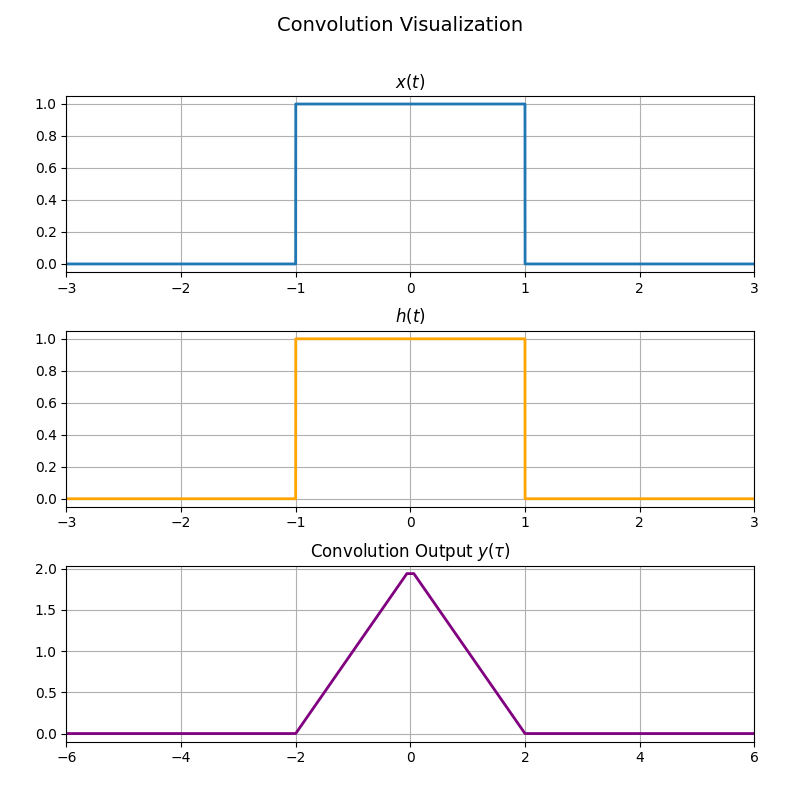
\includegraphics[width=0.7\textwidth]{images/problem_1_2_snapshot.png}
\end{center}
\end{solution}
% ==================== %

\newpage

% === Problem 1.3. === %
\begin{subproblems}[resume]
    \item \( t[u(t)-u(t-1)]*u(t) \)
\end{subproblems}

\begin{solution}
First, we define the functions involved in the convolution:
\[ x(t) = t[u(t) - u(t-1)] = \begin{cases} 0 & t < 0 \\ t & 0 \leq t < 1 \\ 0 & t \geq 1 \end{cases} \]
\[ u(t) = \begin{cases} 0 & t < 0 \\ 1 & t \geq 0 \end{cases} \]

The convolution \( y(t) = x(t) * u(t) \) is given by:
\[ y(t) = \int_{-\infty}^{\infty} x(\tau) u(t - \tau) \, d\tau \]

Evaluating the convolution integral, we find:
\begin{align*}
    y(t) &= \int_{0}^{1} \tau \cdot u(t - \tau) \, d\tau \\
    y(t) &= \int_{0}^{\min(t, 1)} \tau \, d\tau
\end{align*}

Thus,
\[ \boxed{
y(t) = \begin{cases} 
    0 & t < 0 \\
    \frac{t^2}{2} & 0 \leq t < 1 \\
    \frac{1}{2} & t \geq 1
\end{cases}
} \]

Using Python to verify this result, we can implement the convolution and plot the results.
The plot of the signal is shown below:
\begin{center}
    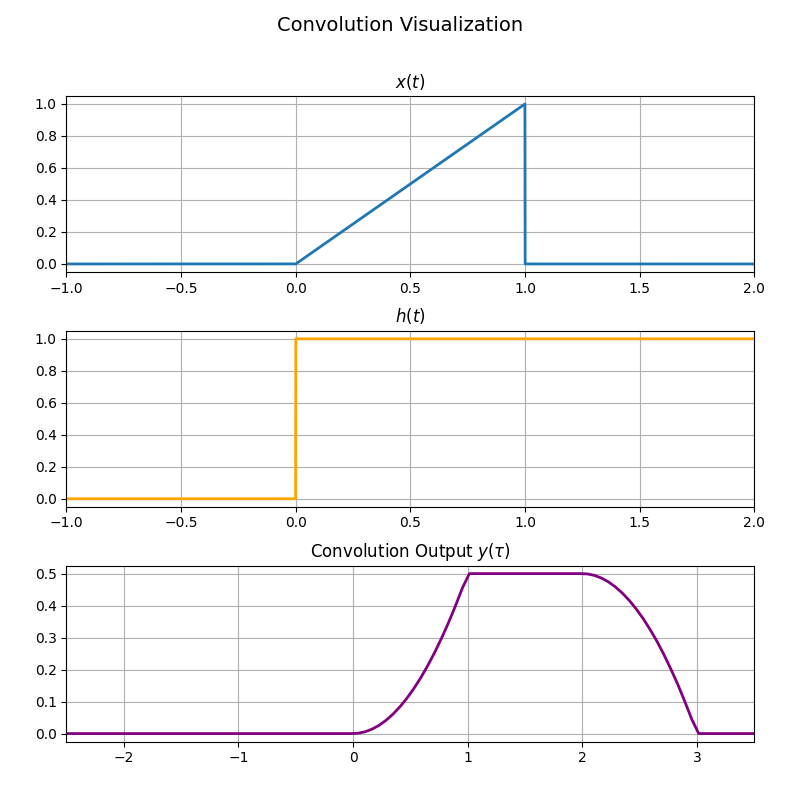
\includegraphics[width=0.7\textwidth]{images/problem_1_3_snapshot.png}
\end{center}
\end{solution}
% ==================== %
% ================================================================================ %

\newpage

% ================================================================================ %
%                                    Problem 02                                    %
% ================================================================================ %
\begin{problem}
Determine the convolution \( y(t) = h(t)*x(t) \) using Graphical Interpretation of the pairs of the signals shown
\end{problem}

\begin{solution}
The convolution \( y(t) = h(t) * x(t) \) can be determined graphically by following these steps:
\begin{enumerate}
    \item Flip one of the signals, typically \( h(t) \), to get \( h(-\tau) \).
    \item Shift the flipped signal by \( t \) to get \( h(t - \tau) \).
    \item For each value of \( t \), calculate the area of overlap between \( x(\tau) \) and \( h(t - \tau) \).
    \item The value of the convolution \( y(t) \) at each \( t \) is the area of overlap calculated in the previous step.
\end{enumerate}
Using Python to visualize and compute the convolution graphically, we can create an animation that demonstrates the convolution process step-by-step.

\vspace{3mm}

The resulting convolution \( y(t) \) is shown in the gif files in \href{https://github.com/patthadon-p/CEDT-2110203-CEM-II/tree/main/signal/homework-2/images}{my GitHub repository} for this homework.
\end{solution}


% === Problem 2.1. === %
\begin{tosubmit}
\begin{subproblems}[start=1]
    \item \submitsolution
\end{subproblems}

Using Python to visualize and compute the convolution graphically,
we can create an animation that demonstrates the convolution process step-by-step
as shown in the gif files in \href{https://github.com/patthadon-p/CEDT-2110203-CEM-II/blob/main/signal/homework-2/images/problem_2_1.gif}{Problem 2.1 Animation}.

\vspace{3mm}

The plot of the signal is shown below:
\begin{center}
    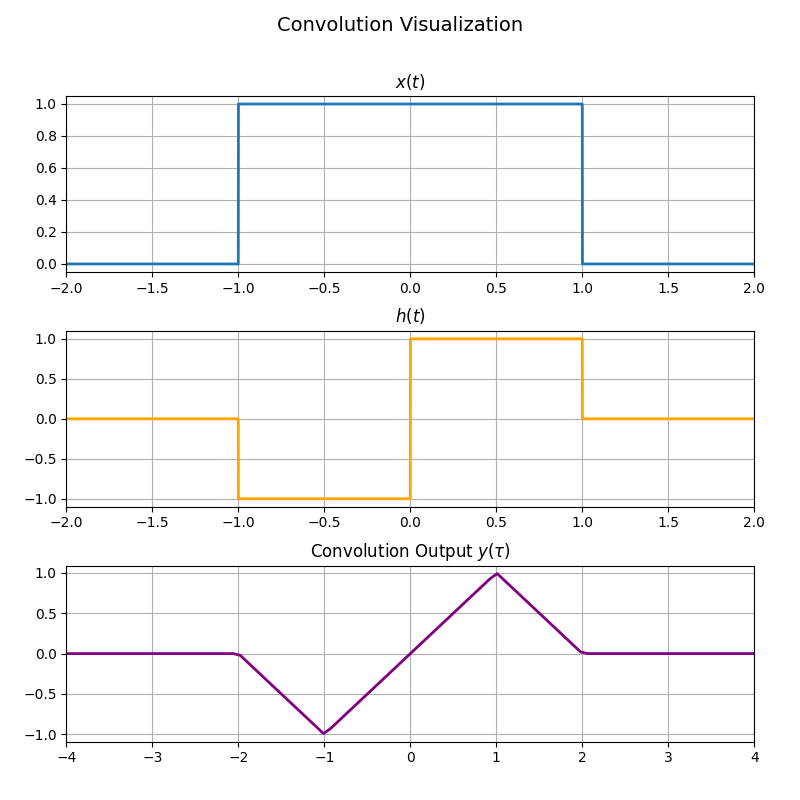
\includegraphics[width=0.75\textwidth]{images/problem_2_1_snapshot.png}
\end{center}
\end{tosubmit}
% ==================== %

\newpage 

% === Problem 2.2. === %
\begin{subproblems}[start=2]
    \item
\end{subproblems}

\begin{solution}
    Using Python to visualize and compute the convolution graphically,
    we can create an animation that demonstrates the convolution process step-by-step
    as shown in the gif files in \href{https://github.com/patthadon-p/CEDT-2110203-CEM-II/blob/main/signal/homework-2/images/problem_2_2.gif}{Problem 2.2 Animation}.
    
    \vspace{3mm}
    
    The plot of the signal is shown below:
    \begin{center}
        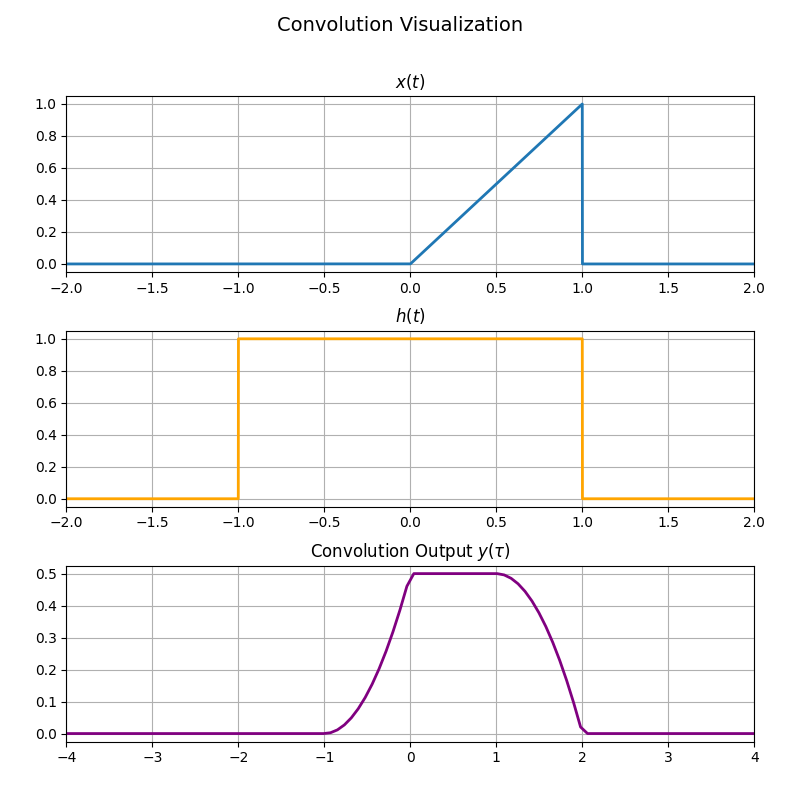
\includegraphics[width=0.75\textwidth]{images/problem_2_2_snapshot.png}
    \end{center}
\end{solution}
% ==================== %

\newpage

% === Problem 2.3. === %
\begin{tosubmit}
\begin{subproblems}[start=3]
    \item \submitsolution
\end{subproblems}

Using Python to visualize and compute the convolution graphically,
we can create an animation that demonstrates the convolution process step-by-step
as shown in the gif files in \href{https://github.com/patthadon-p/CEDT-2110203-CEM-II/blob/main/signal/homework-2/images/problem_2_3.gif}{Problem 2.3 Animation}.

\vspace{3mm}

The plot of the signal is shown below:
\begin{center}
    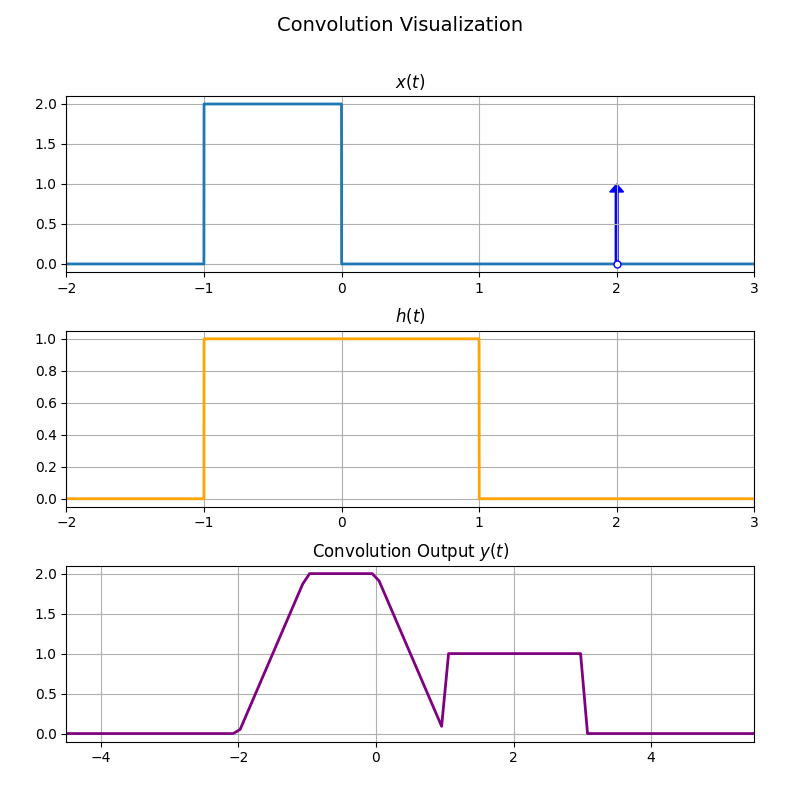
\includegraphics[width=0.75\textwidth]{images/problem_2_3_snapshot.png}
\end{center}
\end{tosubmit}
% ==================== %

\newpage 

% === Problem 2.4. === %
\begin{subproblems}[start=4]
    \item
\end{subproblems}

\begin{solution}
    Using Python to visualize and compute the convolution graphically,
    we can create an animation that demonstrates the convolution process step-by-step
    as shown in the gif files in \href{https://github.com/patthadon-p/CEDT-2110203-CEM-II/blob/main/signal/homework-2/images/problem_2_4.gif}{Problem 2.4 Animation}.
    
    \vspace{3mm}
    
    The plot of the signal is shown below:
    \begin{center}
        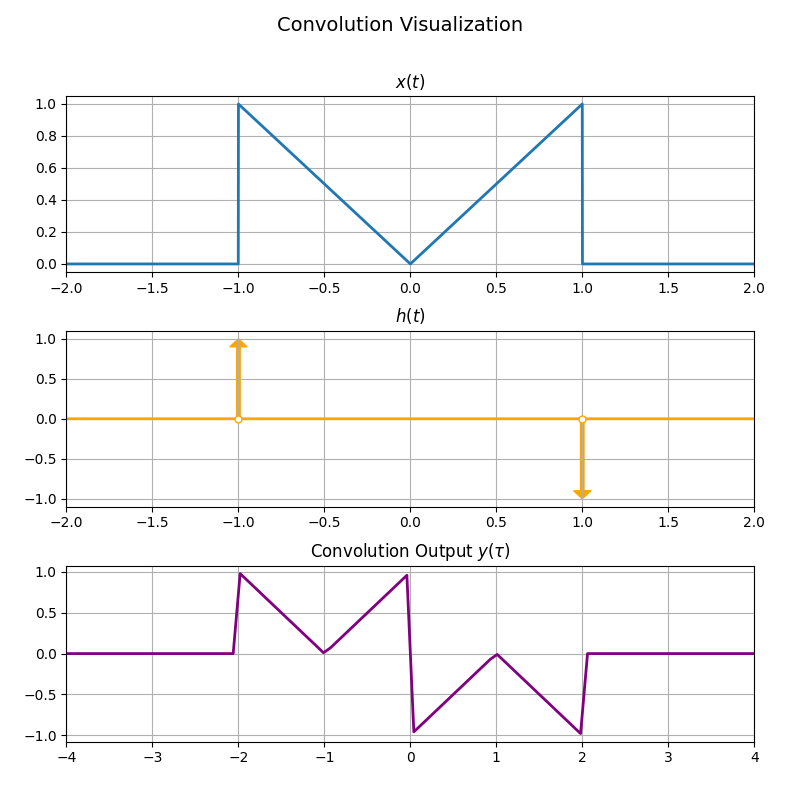
\includegraphics[width=0.75\textwidth]{images/problem_2_4_snapshot.png}
    \end{center}
\end{solution}
% ==================== %
% ================================================================================ %


% ================================================================================ %
%                                    Problem 03                                    %
% ================================================================================ %
\begin{problem}
Let \( f(t) \) and \( g(t) \) be given as follows:
\begin{center}
    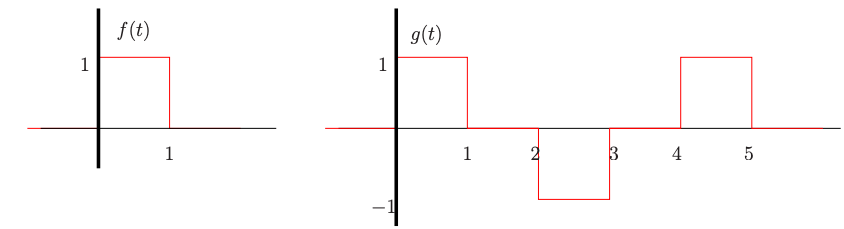
\includegraphics[width=0.8\textwidth]{images/problem_3_reference.png}
\end{center}
\end{problem}


% === Problem 3.1. === %
\begin{subproblems}[start=1]
    \item Sketch the function : \( x(t)$ = $f(t) * g(t) \)
\end{subproblems}

\begin{solution}
Using Python to visualize and compute the convolution graphically,
we can create an animation that demonstrates the convolution process step-by-step
as shown in the gif files in \href{https://github.com/patthadon-p/CEDT-2110203-CEM-II/blob/main/signal/homework-2/images/problem_3_1.gif}{Problem 3.1 Animation}.

\vspace{3mm}

\newpage
The plot of the signal is shown below:
\begin{center}
    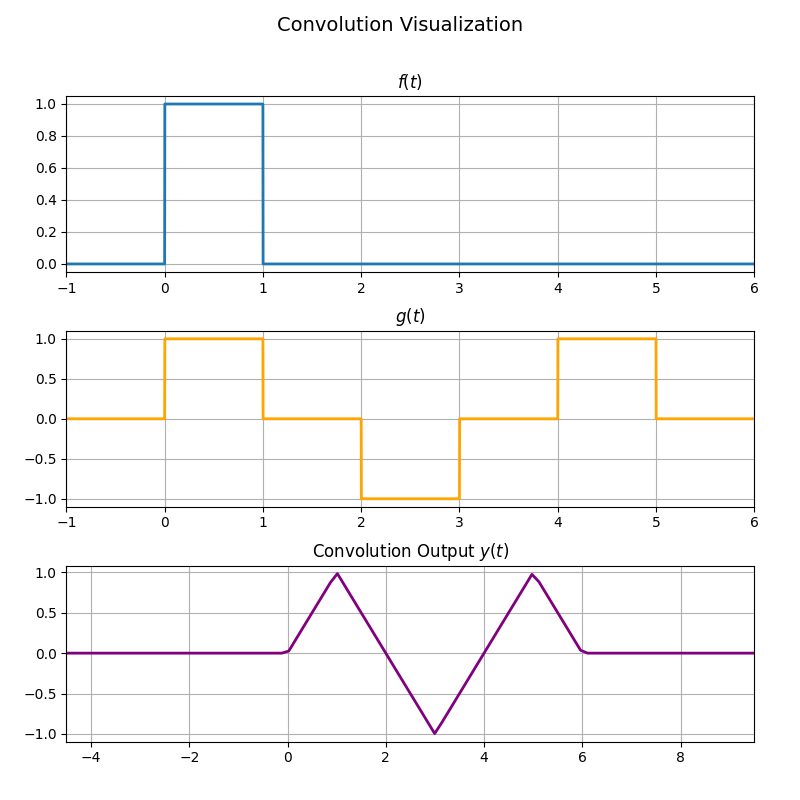
\includegraphics[width=0.75\textwidth]{images/problem_3_1_snapshot.png}
\end{center}
\end{solution}
% ==================== %


% === Problem 3.2. === %
\begin{subproblems}[start=2]
    \item Show that if \( a(t) = b(t) * c(t) \), then \( (Mb(t))*c(t) = Ma(t) \), for any real number \( M \) (hint: use the convolution integral formula)
\end{subproblems}

\begin{solution}
Given that \( a(t) = b(t) * c(t) \), we can express this using the convolution integral:
\[ a(t) = \int_{-\infty}^{\infty} b(\tau) c(t - \tau) \, d\tau \]

Now, we want to show that \( (Mb(t)) * c(t) = Ma(t) \). We start by writing the convolution of \( Mb(t) \) with \( c(t) \):
\[ (Mb(t)) * c(t) = \int_{-\infty}^{\infty} Mb(\tau) c(t - \tau) \, d\tau \]

Factoring out the constant \( M \) from the integral, we have:
\[ (Mb(t)) * c(t) = M \int_{-\infty}^{\infty} b(\tau) c(t - \tau) \, d\tau \]
\[ (Mb(t)) * c(t) = M a(t) \]

Thus, we have shown that:
\[ \boxed{(Mb(t)) * c(t) = Ma(t)} \]
\end{solution}
% ==================== %
% ================================================================================ %

\newpage

% ================================================================================ %
%                                    Problem 04                                    %
% ================================================================================ %
\begin{problem}
Find the convolution \( y[n] = h[n] * x[n] \) of the following signals:
\end{problem}

% === Problem 4.1. === %
\begin{tosubmit}
\begin{subproblems}[start=1]
    \item \( x[n] = \begin{cases} -1 , -5 \leq n \leq -1 \\ 1 , 0 \leq n \leq 4 \end{cases},\, h[n] = 2u[n] \)
\end{subproblems}

\par\noindent\submitsolution
To find the convolution \( y[n] = h[n] * x[n] \), we use the discrete convolution formula:
\[ y[n] = \sum_{k=-\infty}^{\infty} x[k] h[n - k] \]

Consider the value of \( y[n] \):
\begin{align*}
    y[n] &= \sum_{k=-\infty}^{\infty} x[k] h[n - k] \\
    &= \sum_{k=-5}^{-1} x[k] h[n - k] + \sum_{k=0}^{4} x[k] h[n - k] \\
    &= \sum_{k=-5}^{-1} (-1) \cdot 2u[n - k] + \sum_{k=0}^{4} (1) \cdot 2u[n - k] \\
    &= -2 \sqbracket{ \sum_{k=-5}^{-1} u[n - k] - \sum_{k=0}^{4} u[n - k] } \\
    y[n] &= -2 \sqbracket{ \sum_{j=n+1}^{n+5} u[j] - \sum_{j=n-4}^{n} u[j] } \\
\end{align*}

Calculating the convolution for different ranges of \( n \):
\begin{itemize}
    \item For \( -5 \leq n < 0 \):
    \begin{align*}
        y[n] &= -2 \sqbracket{ \sum_{j=n+1}^{n+5} u[j] - \sum_{j=n-4}^{n} u[j] } \\
        &= -2 \sqbracket{ n + 6  } \\
        y[n] &= -2n - 12
    \end{align*}
    \item For \( 0 \leq n < 5 \):
    \begin{align*}
        y[n] &= -2 \sqbracket{ \sum_{j=n+1}^{n+5} u[j] - \sum_{j=n-4}^{n} u[j] } \\
        &= -2 \sqbracket{ 5 - (n - 3) } \\
        y[n] &= 2n - 8
    \end{align*}
\end{itemize}

Thus, the final result of the convolution is:
\[ \boxed{
y[n] = \begin{cases}
-2n - 12 & -5 \leq n < 0 \\
2n - 8 & 0 \leq n < 5 \\
0 & \text{otherwise}
\end{cases}
} \]
\end{tosubmit}
% ==================== %

\newpage

% === Problem 4.2. === %
\begin{subproblems}[start=2]
    \item \( x[n] = u[n],\, h[n] = 1 \; ; 0 \leq n \leq 9 \)
\end{subproblems}

\begin{solution}
To find the convolution \( y[n] = h[n] * x[n] \), we use the discrete convolution formula:
\[ y[n] = \sum_{k=-\infty}^{\infty} x[k] h[n - k] \]

Consider the value of \( y[n] \):
\begin{align*}
    y[n] &= \sum_{k=-\infty}^{\infty} x[k] h[n - k] \\
    &= \sum_{k=0}^{\infty} u[k] \cdot h[n - k] \\
    &= \sum_{k=0}^{\infty} 1 \cdot h[n - k] \\
    y[n] &= \sum_{j=-\infty}^{n} h[j]
\end{align*}

Calculating the convolution for different ranges of \( n \):
\begin{itemize}
    \item For \( 0 \leq n < 9 \):
    \begin{align*}
        y[n] &= \sum_{j=-\infty}^{n} h[j] \\
        &= \sum_{j=0}^{n} 1 \\
        y[n] &= n + 1
    \end{align*}
    \item For \( n \geq 9 \):
    \begin{align*}
        y[n] &= \sum_{j=-\infty}^{n} h[j] \\
        &= \sum_{j=0}^{9} 1 \\
        y[n] &= 10
    \end{align*}
\end{itemize}

Thus, the final result of the convolution is:
\[ \boxed{
y[n] = \begin{cases}
n + 1 & 0 \leq n < 9 \\
10 & n \geq 9 \\
0 & \text{otherwise}
\end{cases}
} \]
\end{solution}
% ==================== %

\newpage

% === Problem 4.3. === %
\begin{tosubmit}    
\begin{subproblems}[start=3]
    \item \( x[n] = \paren{ \frac{1}{2} }^n u[n],\, h[n] = \delta[n] +\delta[n-1] +  \paren{ \frac{1}{3} }^n u[n] \)
\end{subproblems}

\par\noindent\submitsolution
To find the convolution \( y[n] = h[n] * x[n] \), we use the discrete convolution formula:
\[ y[n] = \sum_{k=-\infty}^{\infty} x[k] h[n - k] \]

Consider the value of \( y[n] \):
\begin{align*}
    y[n] &= \sum_{k=-\infty}^{\infty} x[k] h[n - k] \\
    &= \sum_{k=0}^{\infty} \paren{ \frac{1}{2} }^k u[k] \cdot \paren{ \delta[n - k] + \delta[n - k - 1] + \paren{ \frac{1}{3} }^{n - k} u[n - k] } \\
    y[n] &= \sum_{k=0}^{\infty} \paren{ \frac{1}{2} }^k \delta[n - k] + \sum_{k=0}^{\infty} \paren{ \frac{1}{2} }^k \delta[n - k - 1] + \sum_{k=0}^{\infty} \paren{ \frac{1}{2} }^k \paren{ \frac{1}{3} }^{n - k} u[n - k] \\
\end{align*}

Calculating the convolution for different ranges of \( n \):
\begin{itemize}
    \item For \( n \geq 0 \):
    \begin{align*}
        y[n] &= \sum_{k=0}^{\infty} \paren{ \frac{1}{2} }^k \delta[n - k] + \sum_{k=0}^{\infty} \paren{ \frac{1}{2} }^k \delta[n - k - 1] + \sum_{k=0}^{\infty} \paren{ \frac{1}{2} }^k \paren{ \frac{1}{3} }^{n - k} u[n - k] \\
        &= \paren{ \frac{1}{2} }^n + \paren{ \frac{1}{2} }^{n-1} + \sum_{k=0}^{n} \paren{ \frac{1}{2} }^k \paren{ \frac{1}{3} }^{n - k} \\
        &= \paren{ \frac{1}{2} }^n + 2 \paren{ \frac{1}{2} }^n + \paren{ \frac{1}{3} }^n \sum_{k=0}^{n} \paren{ \frac{3}{2} }^k \\
        &= 3 \paren{ \frac{1}{2} }^n + \paren{ \frac{1}{3} }^n \frac{1 - \paren{ \frac{3}{2} }^{n+1}}{1 - \frac{3}{2}} \\
        &= 3 \paren{ \frac{1}{2} }^n + \paren{ \frac{1}{3} }^n (-2)\paren{ 1 - \paren{ \frac{3}{2} }^{n+1}} \\
        &= 3 \paren{ \frac{1}{2} }^n + (-2) \paren{ \frac{1}{3} }^{n} + 3 \paren{ \frac{1}{2} }^{n} \\
        y[n] &= 6 \paren{ \frac{1}{2} }^n - 2 \paren{ \frac{1}{3} }^{n} \\
    \end{align*}
\end{itemize}

Thus, the final result of the convolution is:
\[ \boxed{
y[n] = \begin{cases}
6 \paren{ \frac{1}{2} }^n - 2 \paren{ \frac{1}{3} }^n & n \geq 0 \\
0 & \text{otherwise}
\end{cases}
} \]
\end{tosubmit}
% ==================== %

\newpage

% === Problem 4.4. === %
\begin{subproblems}[start=4]
    \item \( x[n] = \paren{ \frac{1}{3} }^n u[n],\, h[n] = \delta[n] + \paren{ \frac{1}{2} }^n u[n] \)
\end{subproblems}

\begin{solution}
To find the convolution \( y[n] = h[n] * x[n] \), we use the discrete convolution formula:
\[ y[n] = \sum_{k=-\infty}^{\infty} x[k] h[n - k] \]

Consider the value of \( y[n] \):
\begin{align*}
    y[n] &= \sum_{k=-\infty}^{\infty} x[k] h[n - k] \\
    &= \sum_{k=0}^{\infty} \paren{ \frac{1}{3} }^k u[k] \cdot \paren{ \delta[n - k] + \paren{ \frac{1}{2} }^{n - k} u[n - k] } \\
    y[n] &= \sum_{k=0}^{\infty} \paren{ \frac{1}{3} }^k \delta[n - k] + \sum_{k=0}^{\infty} \paren{ \frac{1}{3} }^k \paren{ \frac{1}{2} }^{n - k} u[n - k] \\
\end{align*}

Calculating the convolution for different ranges of \( n \):
\begin{itemize}
    \item For \( n \geq 0 \):
    \begin{align*}
        y[n] &= \sum_{k=0}^{\infty} \paren{ \frac{1}{3} }^k \delta[n - k] + \sum_{k=0}^{\infty} \paren{ \frac{1}{3} }^k \paren{ \frac{1}{2} }^{n - k} u[n - k] \\
        &= \paren{ \frac{1}{3} }^n + \sum_{k=0}^{n} \paren{ \frac{1}{3} }^k \paren{ \frac{1}{2} }^{n - k} \\
        &= \paren{ \frac{1}{3} }^n + \paren{ \frac{1}{2} }^n \sum_{k=0}^{n} \paren{ \frac{2}{3} }^k \\
        &= \paren{ \frac{1}{3} }^n + \paren{ \frac{1}{2} }^n \cdot \frac{1 - \paren{ \frac{2}{3} }^{n+1}}{1 - \frac{2}{3}} \\
        &= \paren{ \frac{1}{3} }^n + 3 \paren{ \frac{1}{2} }^n \sqbracket{ 1 - \paren{ \frac{2}{3} }^{n+1} } \\
        &= \paren{ \frac{1}{3} }^n + 3 \paren{ \frac{1}{2} }^n - 2 \paren{ \frac{1}{3} }^{n} \\
        y[n] &= 3 \paren{ \frac{1}{2} }^n - \paren{ \frac{1}{3} }^{n} \\
    \end{align*}
\end{itemize}

Thus, the final result of the convolution is:
\[ \boxed{
y[n] = \begin{cases}
3 \paren{ \frac{1}{2} }^n - \paren{ \frac{1}{3} }^n & n \geq 0 \\
0 & \text{otherwise}
\end{cases}
} \]
\end{solution}
% ==================== %
% ================================================================================ %


\end{document}